\chapter{Pipeline}

\section{Motivations}
As discussed before, an instruction finishes within a single clock cycle. However, this can be inefficient since the clock cycle must be timed to accommodate the slowest instruction, meaning every instruction takes the same amount of time. This results in wasted area, as some functional units (e.g., adders) must be duplicated since they cannot be shared within a single clock cycle. Additionally, for simple instructions, the latter part of the clock cycle might be wasted.

\begin{eg}
  Calculate the cycle time assuming negligible delays (for muxes, control unit, sign extension, PC access, shift left by 2, wires) except for:

  - Instruction fetch and update PC (IF), read/write data from/to data memory (MEM) (4 ns)

  - Execute R-type; calculate memory address (EXE) (2 ns)

  - Register fetch and instruction decode (ID), write the result data into the register file (WB) (1 ns)

  \textbf{Solution:} 
  \begin{table}[H]
    \centering
    \begin{tabular}{c|c|c|c|c|c|c}
        \toprule
        Instruction & IF & ID & EXE & MEM & WB &  Total \\
      \midrule
        R / I type & 4 & 1 & 2 &  & 1 & 8  \\
        \verb|lw| & 4 & 1 & 2 & 4 & 1 & 12  \\
        \verb|sw| & 4 & 1 & 2 & 4 &  & 11  \\
        \verb|beq| & 4 & 1 & 2 &  &  & 7  \\
      \midrule
        \verb|jal| & 4 & 1 & 2 &  & 1 & 8  \\
        \verb|jalr| & 4 & 1 & 2 &  & 1 & 9  \\
        \bottomrule
    \end{tabular}
  \end{table}
\end{eg}

Therefore, we try to make it faster by fetching and executing the next instructions while the current instruction is running, and we introduce the concept of pipelining here. Under ideal conditions, with a large number of instructions, the speedup from pipelining is approximately equal to the number of pipeline stages. For example, a five-stage pipeline is nearly five times faster because the clock cycle is ``nearly'' five times faster.

Also, we have
\[
\text{CPU time} = \text{CPI} \times \text{CC} \times \text{IC},
\]
where CPI = cycles per instruction, CC = clock cycle time, and IC = instruction count.

By pipelining, it reduces the time spent on each clock cycle and decreases the CPU time.

\section{Pipeline Basis}
Instructions are divided into five stages:

- IF: Instruction fetch and PC update

- ID: Instruction decode and register file read

- EXE: Execution or address calculation

- MEM: Data memory access

- WB: Write the result data back into the register file

By dividing the stages, we can increase the total amount of work done in a given time. However, instruction latency, which is the time from the start of an instruction to its completion, is not reduced.

Similarly, the clock cycle is limited by the slowest stage, so some stages do not need the whole clock cycle.

This might lead to the situation where, for example, if we have IF = 100ps, ID = 100ps, EXE = 200ps, MEM = 200ps, and WB = 100ps, the latency of an instruction takes 1000ps in a pipelined case, while it takes 700ps in a non-pipelined case. However, for more instructions, the overall speed is faster in the pipelined case than in the non-pipelined case.

In RISC-V, the implementation of the pipeline is relatively simple for the following reasons:

1. All instructions have the same length.

2. There are few instruction formats with symmetry across formats.

3. Memory operations occur only in loads and stores.

4. Each instruction writes at most one result, and it does so in the last few pipeline stages.

5. Operands must be aligned in memory, so a single data transfer takes only one data memory access, which is accomplished in RISC-V fields.

\begin{center}
  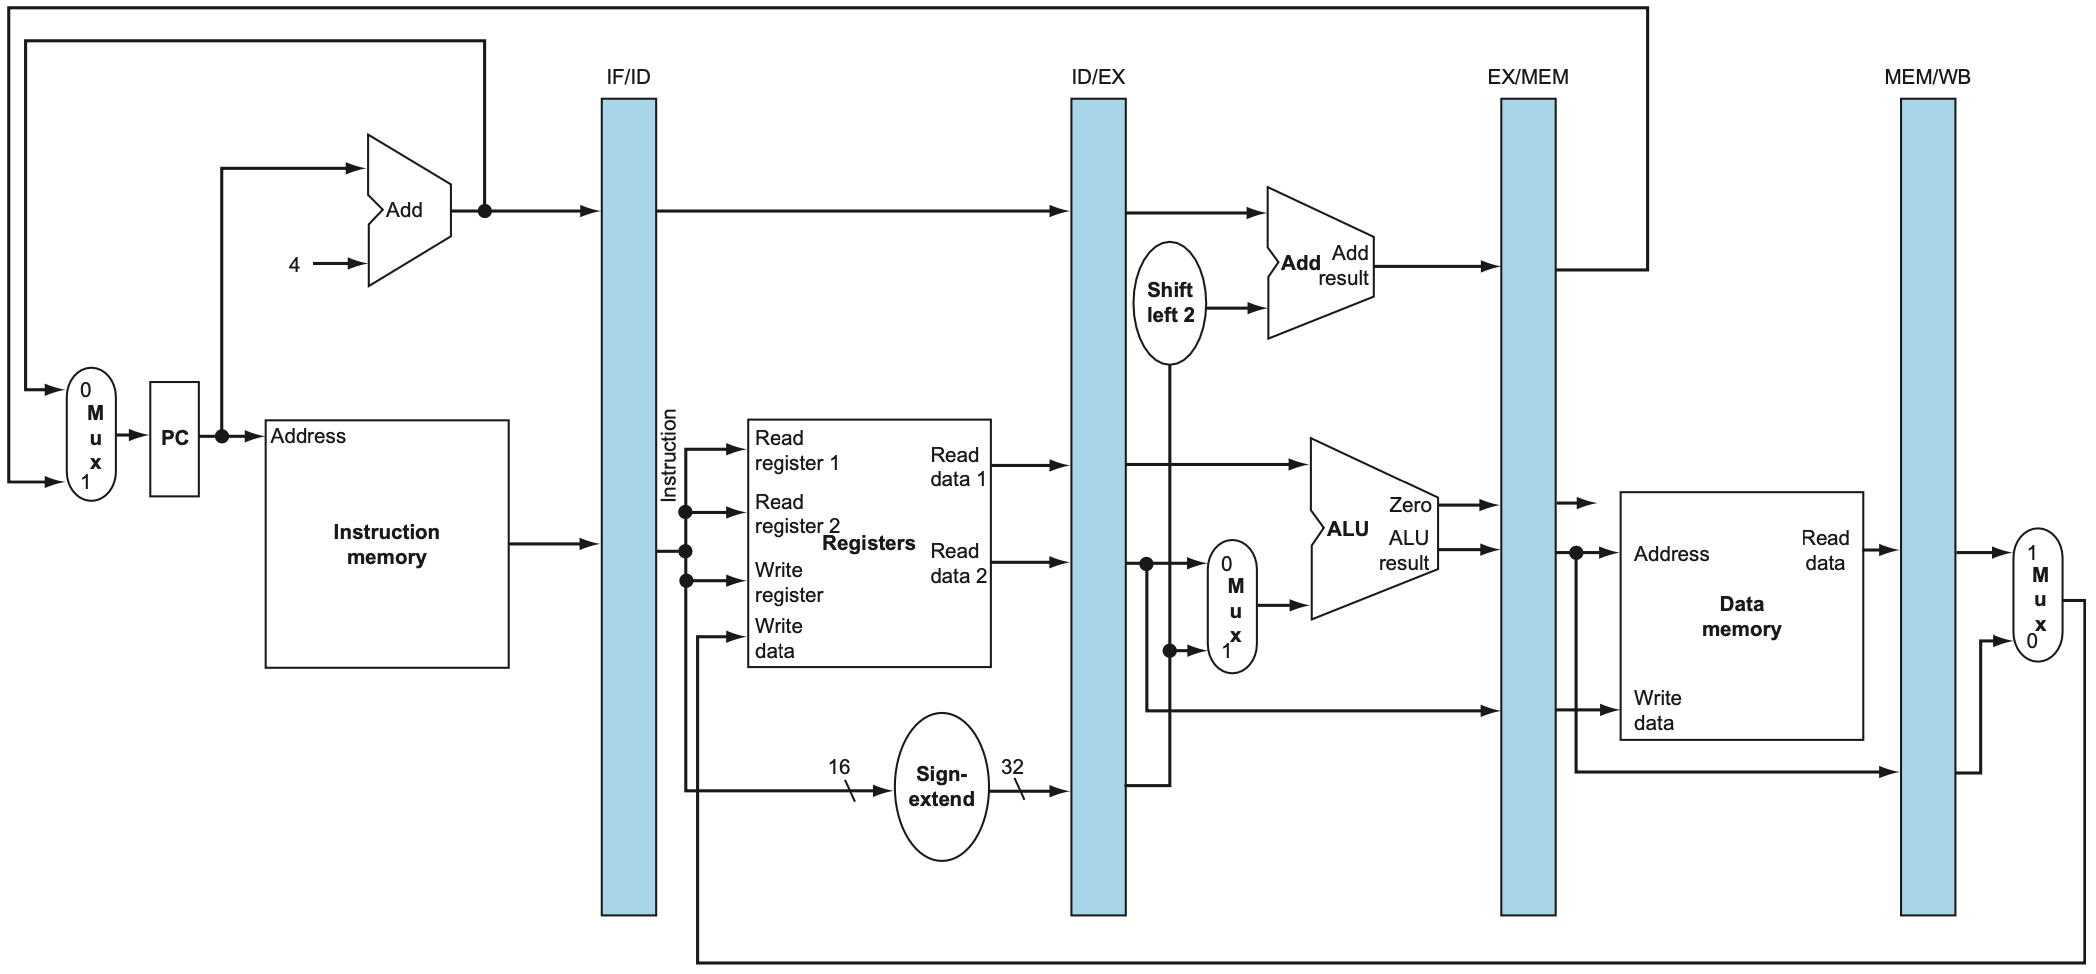
\includegraphics[width=\textwidth]{Figure/Pipeline_reg.png}
\end{center}

State registers are placed between each pipeline stage to isolate them. Each register is a flip-flop, and data moves in at the rising edge. After the pipeline is fully utilized, we can complete one instruction per cycle.

To simplify, we use graphics to represent the RISC-V pipeline.
\begin{center}
  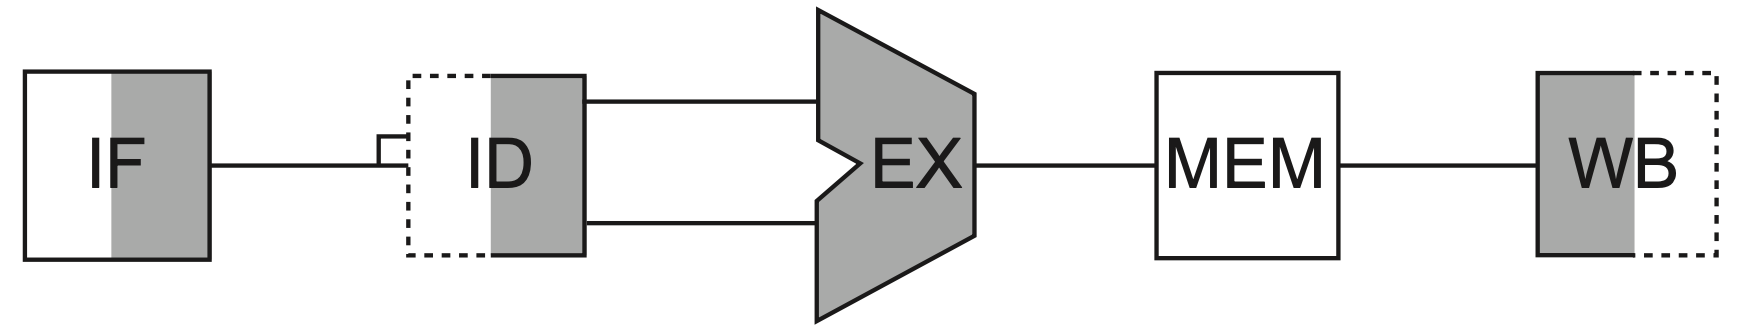
\includegraphics[width=0.4\textwidth]{Figure/Pipeline_graphic.png}
\end{center}

Other pipeline structures are also possible.

We use pipelines because they are better for performance. Once the pipeline is full, one instruction is completed per cycle, so the CPI (cycles per instruction) is 1.

However, pipelines can cause issues, as they may introduce hazards. There are three possible pipeline hazards: structural hazards, caused by a busy resource; data hazards, where data is attempted to be used before it is ready; and control hazards, where control actions depend on the outcome of a previous instruction.

We typically resolve these hazards by allowing pipeline control to detect the hazards and take action to resolve them.

\section{Structural Hazards}
Structural hazards are caused by conflicts in the use of a resource. In a RISC-V pipeline with a single memory, it needs to access both data and instructions to load or store data and fetch new instructions. Therefore, the pipeline datapaths require separate instruction and data memories to avoid such conflicts. 

To resolve a structural hazard, we can provide additional hardware components.

\begin{center}
  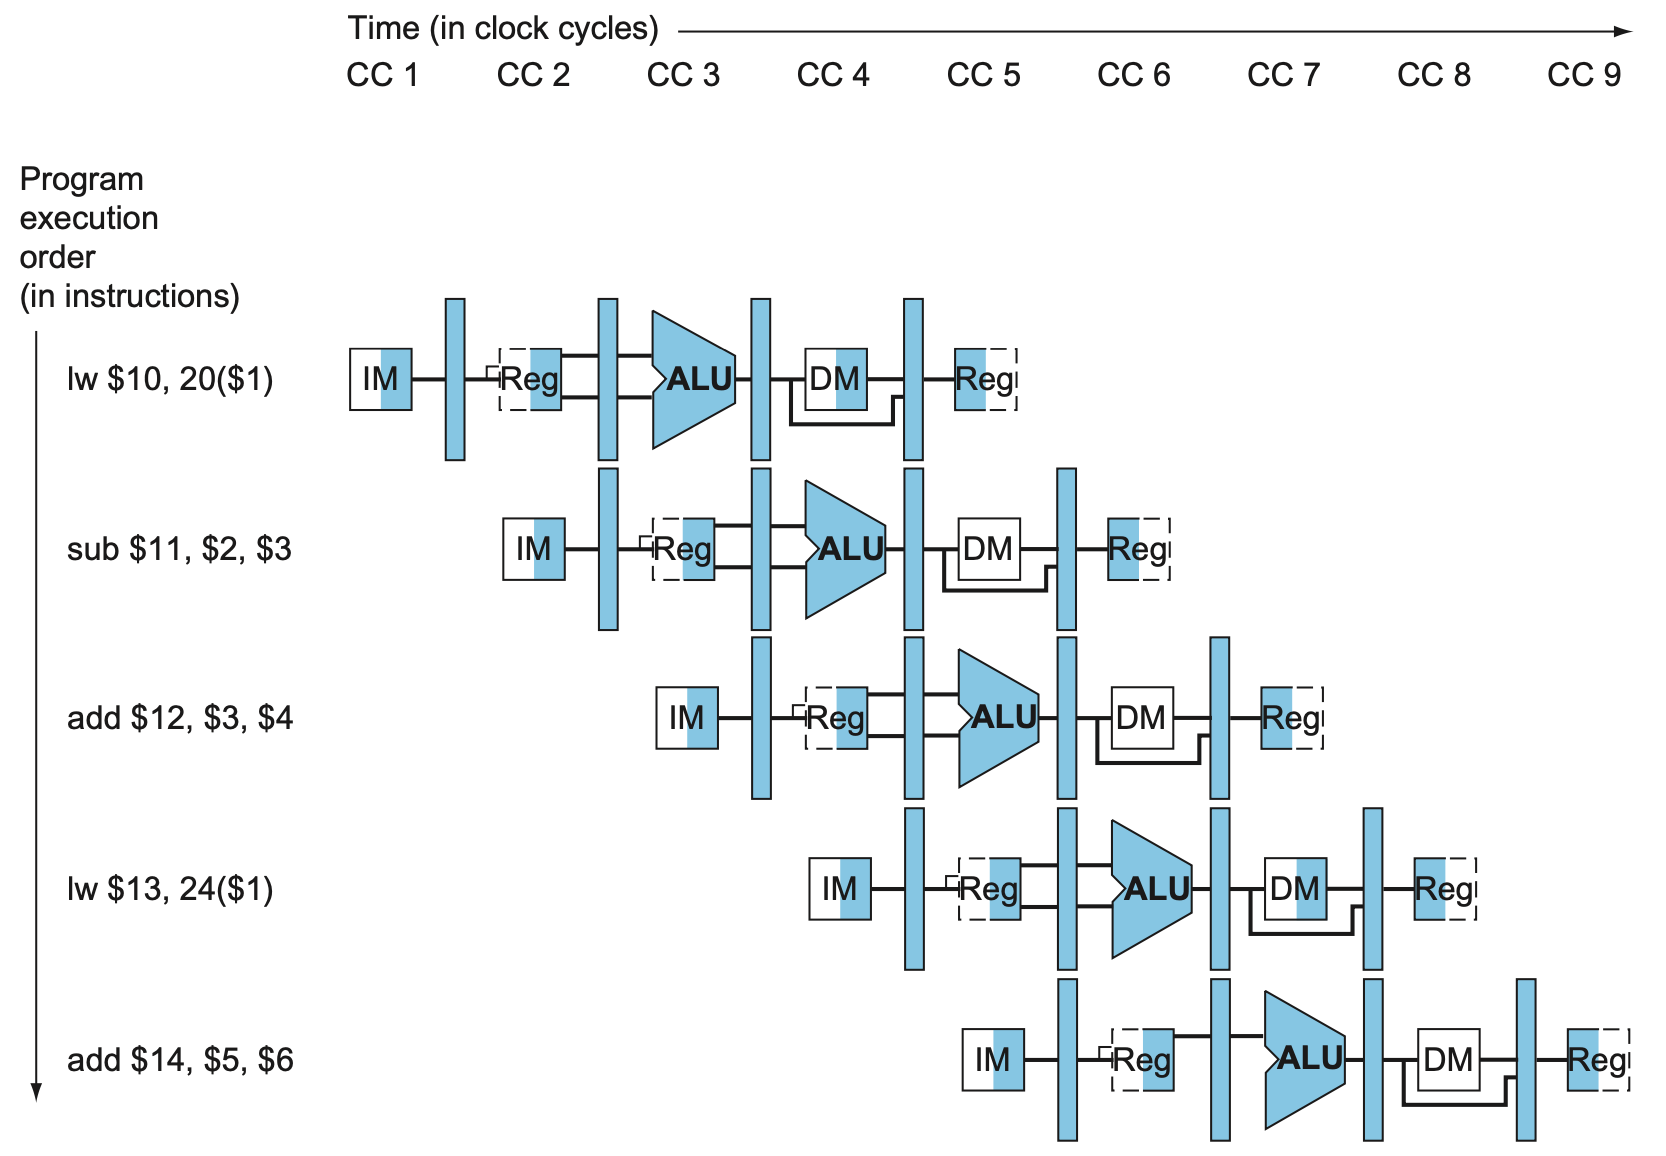
\includegraphics[width=0.8\textwidth]{Figure/structuralHazard.png}
\end{center}

As mentioned above, by separating instruction and data memories, we can resolve the structural hazard. For example, in the diagram above, while the first \verb|lw| is reading data from memory, the second \verb|lw| is reading instructions from memory. Since the memories are separated, the issue is resolved. 

In the diagram above, \verb|sub| and the second \verb|add| instructions are accessing the same register file, which could lead to a structural hazard. This can be fixed by performing reads in the second half of the cycle and writes in the first half. We use the clock edge to control the register writing and loading.

\section{Clocking Methodology}
Clocking methodology defines when signals can be read and when they can be written. The clock rate is given by:
\[
  \text{Clock rate} = \frac{1}{\text{Clock cycle time}}
\]
This can be implemented using level-sensitive latches, master-slave flip-flops, or edge-triggered flip-flops.

The change of state is based on the clock. For latches, the output changes whenever the inputs change and the clock is asserted (level-sensitive methodology). For flip-flops, the output changes only on a clock edge (edge-triggered methodology). 